\chapter{Implementation}

This chapter deals with the description of implementing and modifying the LCS.

For this thesis there was created a test project in the Infomedia TFS where I could do my work. This was so that I would not mess up Infomedia's inflow while trying to make the algorithms work correctly.

First off the Cosine algorithm was implemented in said test project, and then the basic implementation of LCS was implemented.

Then the basic LCS algorithm was implemented in the project, to be used for further development.

\lstset{style=sharpc}
\begin{lstlisting}[caption=Basic LCS implementation in C$^\sharp$, captionpos=b]

public int LongestCommonSubstring(string str1,
	 string str2)
{
    if (String.IsNullOrEmpty(str1) 
    	|| String.IsNullOrEmpty(str2))
    return 0;
	
	int[,] num = new int[str1.Length, str2.Length];
	int maxlen = 0;

    for (int i = 0; i < str1.Length; i++)
  	{
    	for (int j = 0; j < str2.Length; j++)
        {
        	if (str1[i] != str2[j])
            	num[i, j] = 0;
            else
            {
            	if ((i == 0) || (j == 0))
                	num[i, j] = 1;
                else
                    num[i, j] = 1 + num[i - 1, j - 1];

                    if (num[i, j] > maxlen)
                    {
                    	maxlen = num[i, j];
                  	}
           	}
     	}
	}
    return maxlen;
}

\end{lstlisting}

The LCS works by taking in two strings as arguments and then comparing them character by character (see Figure 3.4). This works really well for finding substrings that can have been obfuscated in long lines of text. How ever in this thesis, the main objective is to find substrings of plain words rather than finding bits and pieces.

When comparing two articles with the LCS, the algorithm finds a lot of substrings, but only keeps the longest by default
\begin{figure}
	\centering
	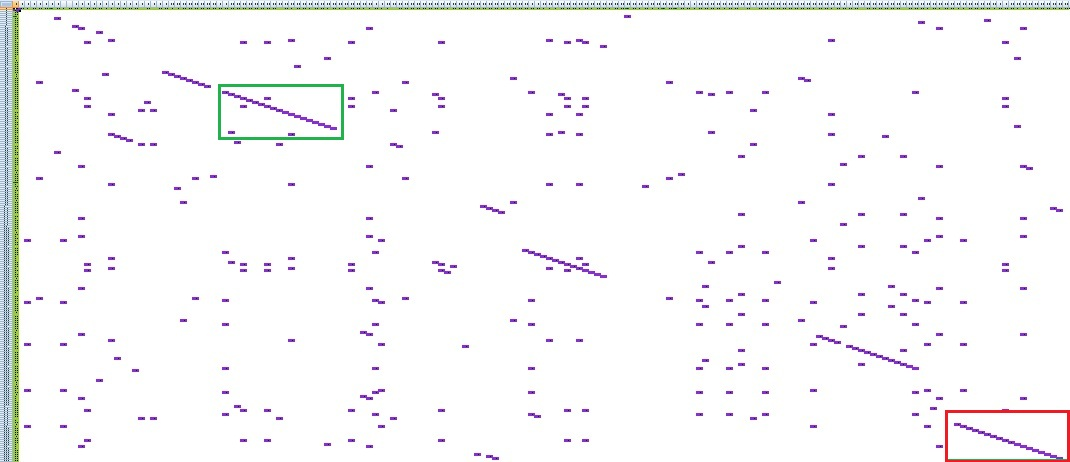
\includegraphics[scale=0.4]{figures/LcsExample}
	\caption{Diagram showing the result of two article being compared by using LCS. See Appendix A.1 for bigger image. The green and red boxes indicates longest common substrings found.}
	\label{LcsEx}
\end{figure}

The green rows seen in Figure ~\ref{LcsEx} is an article (one article along the y-axis and one along the x-axis) split into words (in the basic implementation the articles would be split in characters as seen in figure 3.4, this figure is from the updated version of LCS). All the purple boxes indicates where a match has been found, a diagonal line indicates a row of matches. The longest one would be the \textit{'Longest Common Substring'} and the length of that would be returned by the algorithm. In the example from Figure ~\ref{LcsEx} there are two substrings of equal length (each having a length of 19 words (in the basic LCS the length would the number of characters, including white spaces)), how ever as LCS only returns the length of a single longest common substring (the longest found) and the second one (marked in the red box) is same length, LCS returns the length of the first (marked in the green box) substring. Again, as this example is made out of words rather than characters, the result could vary in case of counting actual characters, but for demonstration purposes the figure explains the idea.

In the case of a perfect match (require both articles to be of the exact same length). A line along the diagonal will be drawn.

\begin{figure}
	\centering
	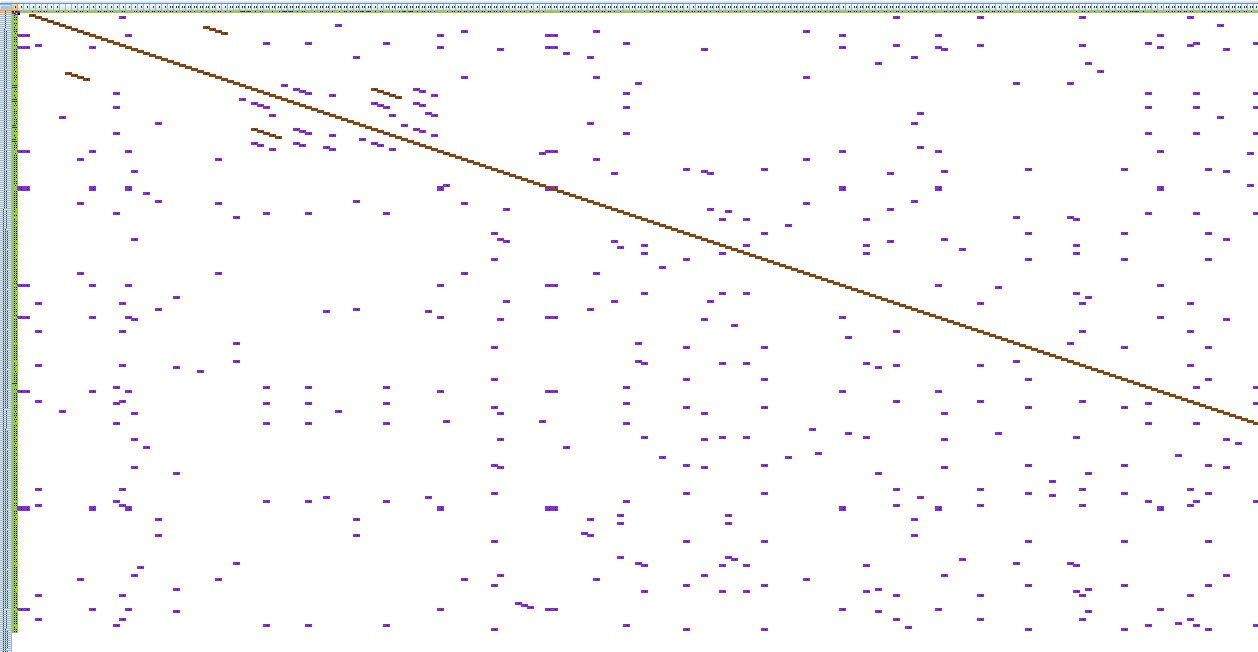
\includegraphics[scale=0.4]{figures/PerfectMatch}
	\caption{Diagram showing a part of an almost perfect match (the article along the y-axis is slightly longer than the article along the x-axis)}
	\label{Match}
\end{figure}

In Figure ~\ref{Match} there is two article that are almost 100\% identical. One of the articles ~\cite{JV1} is slightly shorter than the other article \cite{Lemvig1}. The on line content of the second article is protected by a payment wall, the article content can be found in Appendix B.

The next step was to modify the LCS algorithm to make suit the needs of this thesis. When looking at article duplicates, it makes more sense to look for entire words rather than single characters. This is because when an article is duplicated, any obfuscation or alteration would be done by cutting out sections of the article or moving sections around or adding new sections.



